\documentclass[11pt]{article}

\usepackage[margin=1in]{geometry}
\usepackage{booktabs}
\usepackage{graphicx}
\usepackage{amsmath}
\usepackage{xeCJK}
\usepackage{microtype}
\usepackage{hyperref}

\setCJKmainfont{SimSun}
\setmainfont{Times New Roman}

\title{真实焦栈层间配准敏感性报告}
\author{SRTP Optical Mechanism Analysis}
\date{2026-06-22}

\begin{document}
\maketitle

\section{Research Question}

上一轮真实焦栈分析发现，100um key-texture sample 中存在两类无参考不可靠性：右侧高亮边缘对应早层饱和，普通/暗区存在 DFF peak layer 的局部跳变。一个必须排除的替代解释是：这些现象可能主要来自焦栈采集过程中的层间平移或视野漂移。本轮实验检查真实焦栈不同层之间是否存在显著全局平移，以及平移配准后 DFF peak layer、spike proxy 和 quality proxy 是否发生本质改变。

\section{Method}

读取 40 层真实焦栈并缩放到 $512 \times 640$。使用第 20 层作为参考层，在裁掉两侧高亮边缘后的中心区域上做 phase cross-correlation，估计每层相对参考层的亚像素平移。随后对每层图像做相应平移校正，再分别计算配准前后的 DFF peak layer、spike proxy、low margin、focus entropy、saturation persistence 和 quality proxy。

相位相关返回的 registration error 在该强离焦焦栈中不稳定，本报告不把它作为质量指标，只使用估计位移量与配准前后诊断图变化作为判断依据。

\section{Shift Results}

\begin{table}[htbp]
\centering
\begin{tabular}{lr}
\toprule
Metric & Value \\
\midrule
Max shift magnitude & 0.1118 px \\
Median shift magnitude & 0.0000 px \\
X shift range & -0.1000 to 0.0500 px \\
Y shift range & -0.0500 to 0.0500 px \\
\bottomrule
\end{tabular}
\caption{Estimated global inter-layer translation.}
\end{table}

\begin{figure}[htbp]
\centering
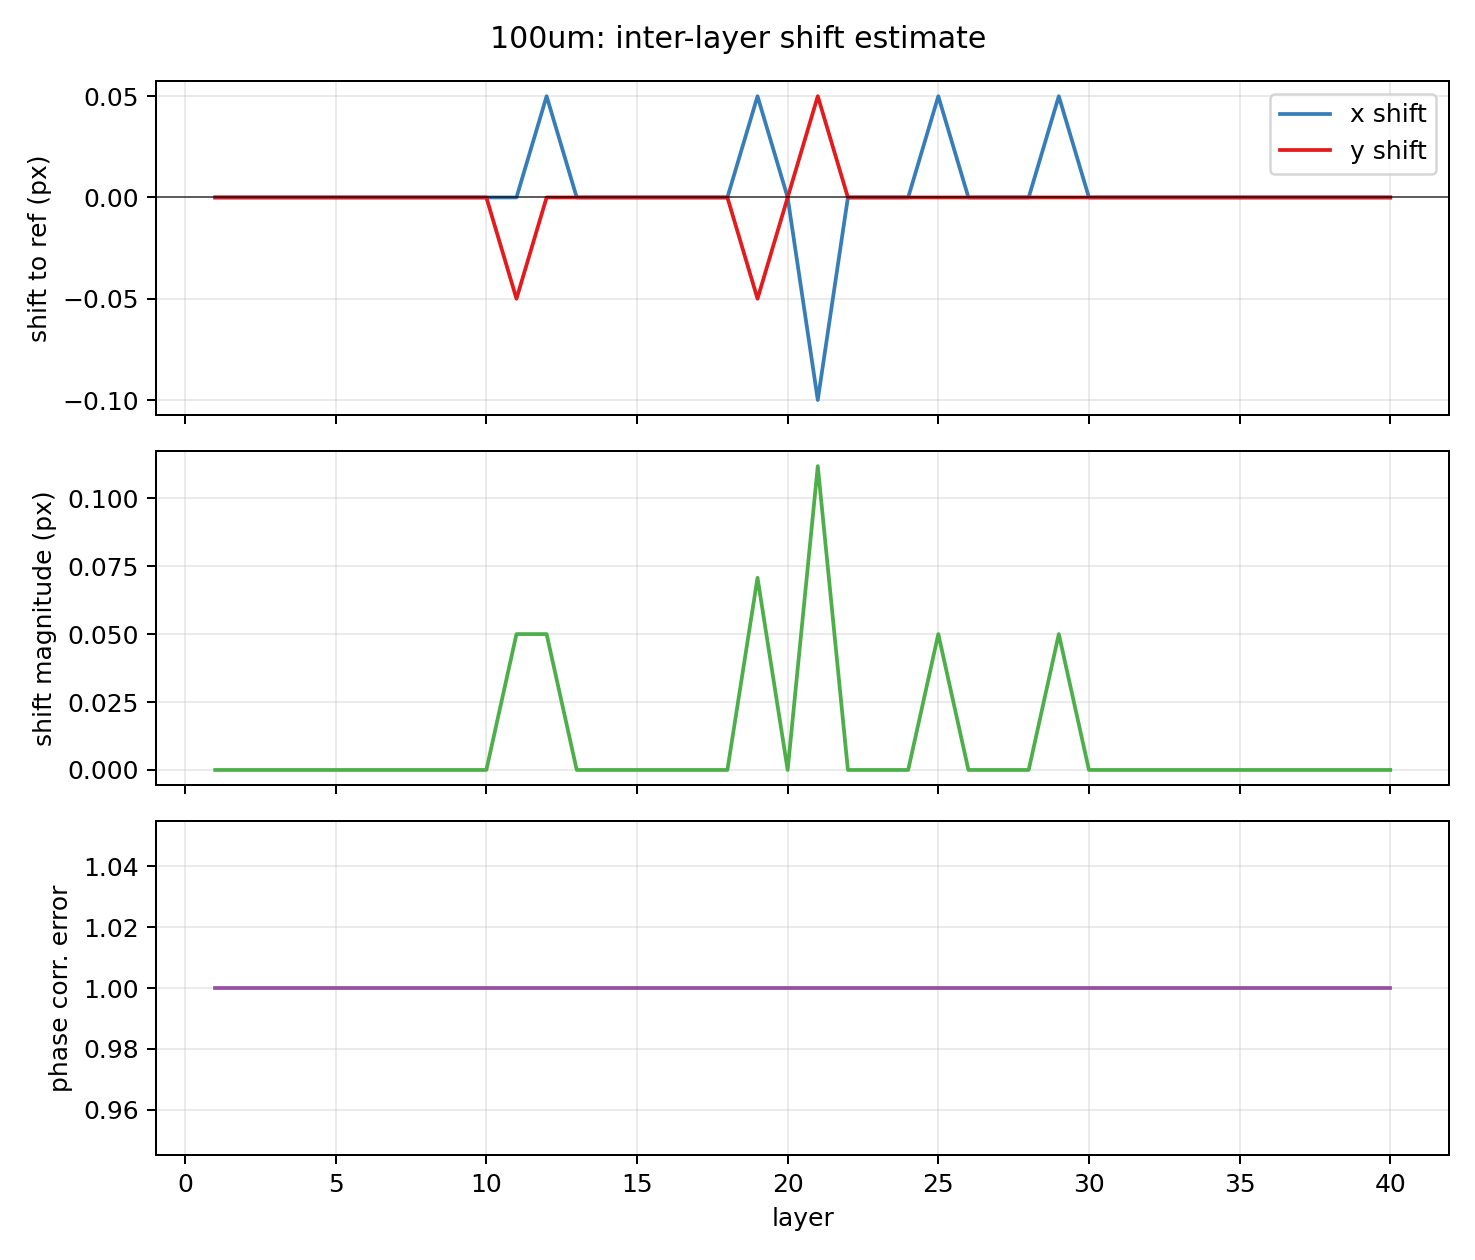
\includegraphics[width=0.86\linewidth]{real_registration_probe/钥匙纹路100um_registration_shifts.png}
\caption{Estimated inter-layer shifts relative to layer 20.}
\end{figure}

\section{Registration Sensitivity}

\begin{table}[htbp]
\centering
\small
\begin{tabular}{lr}
\toprule
Metric & Value \\
\midrule
\texttt{peak\_layer\_changed\_fraction} & 0.0468 \\
\texttt{peak\_layer\_mean\_abs\_change} & 0.3875 \\
\texttt{peak\_layer\_p90\_abs\_change} & 0.0000 \\
\texttt{spike\_proxy\_mean\_before} & 0.0995 \\
\texttt{spike\_proxy\_mean\_after} & 0.1041 \\
\texttt{spike\_proxy\_pearson\_before\_after} & 0.9478 \\
\texttt{quality\_proxy\_mean\_before} & 0.6375 \\
\texttt{quality\_proxy\_mean\_after} & 0.5976 \\
\texttt{quality\_proxy\_pearson\_before\_after} & 0.9825 \\
\texttt{low\_margin\_auc\_spike\_top10\_before} & 0.7293 \\
\texttt{low\_margin\_auc\_spike\_top10\_after} & 0.7287 \\
\texttt{quality\_proxy\_auc\_spike\_top10\_before} & 0.9289 \\
\texttt{quality\_proxy\_auc\_spike\_top10\_after} & 0.9299 \\
\bottomrule
\end{tabular}
\caption{DFF diagnostic sensitivity before and after translation compensation.}
\end{table}

\begin{figure}[htbp]
\centering
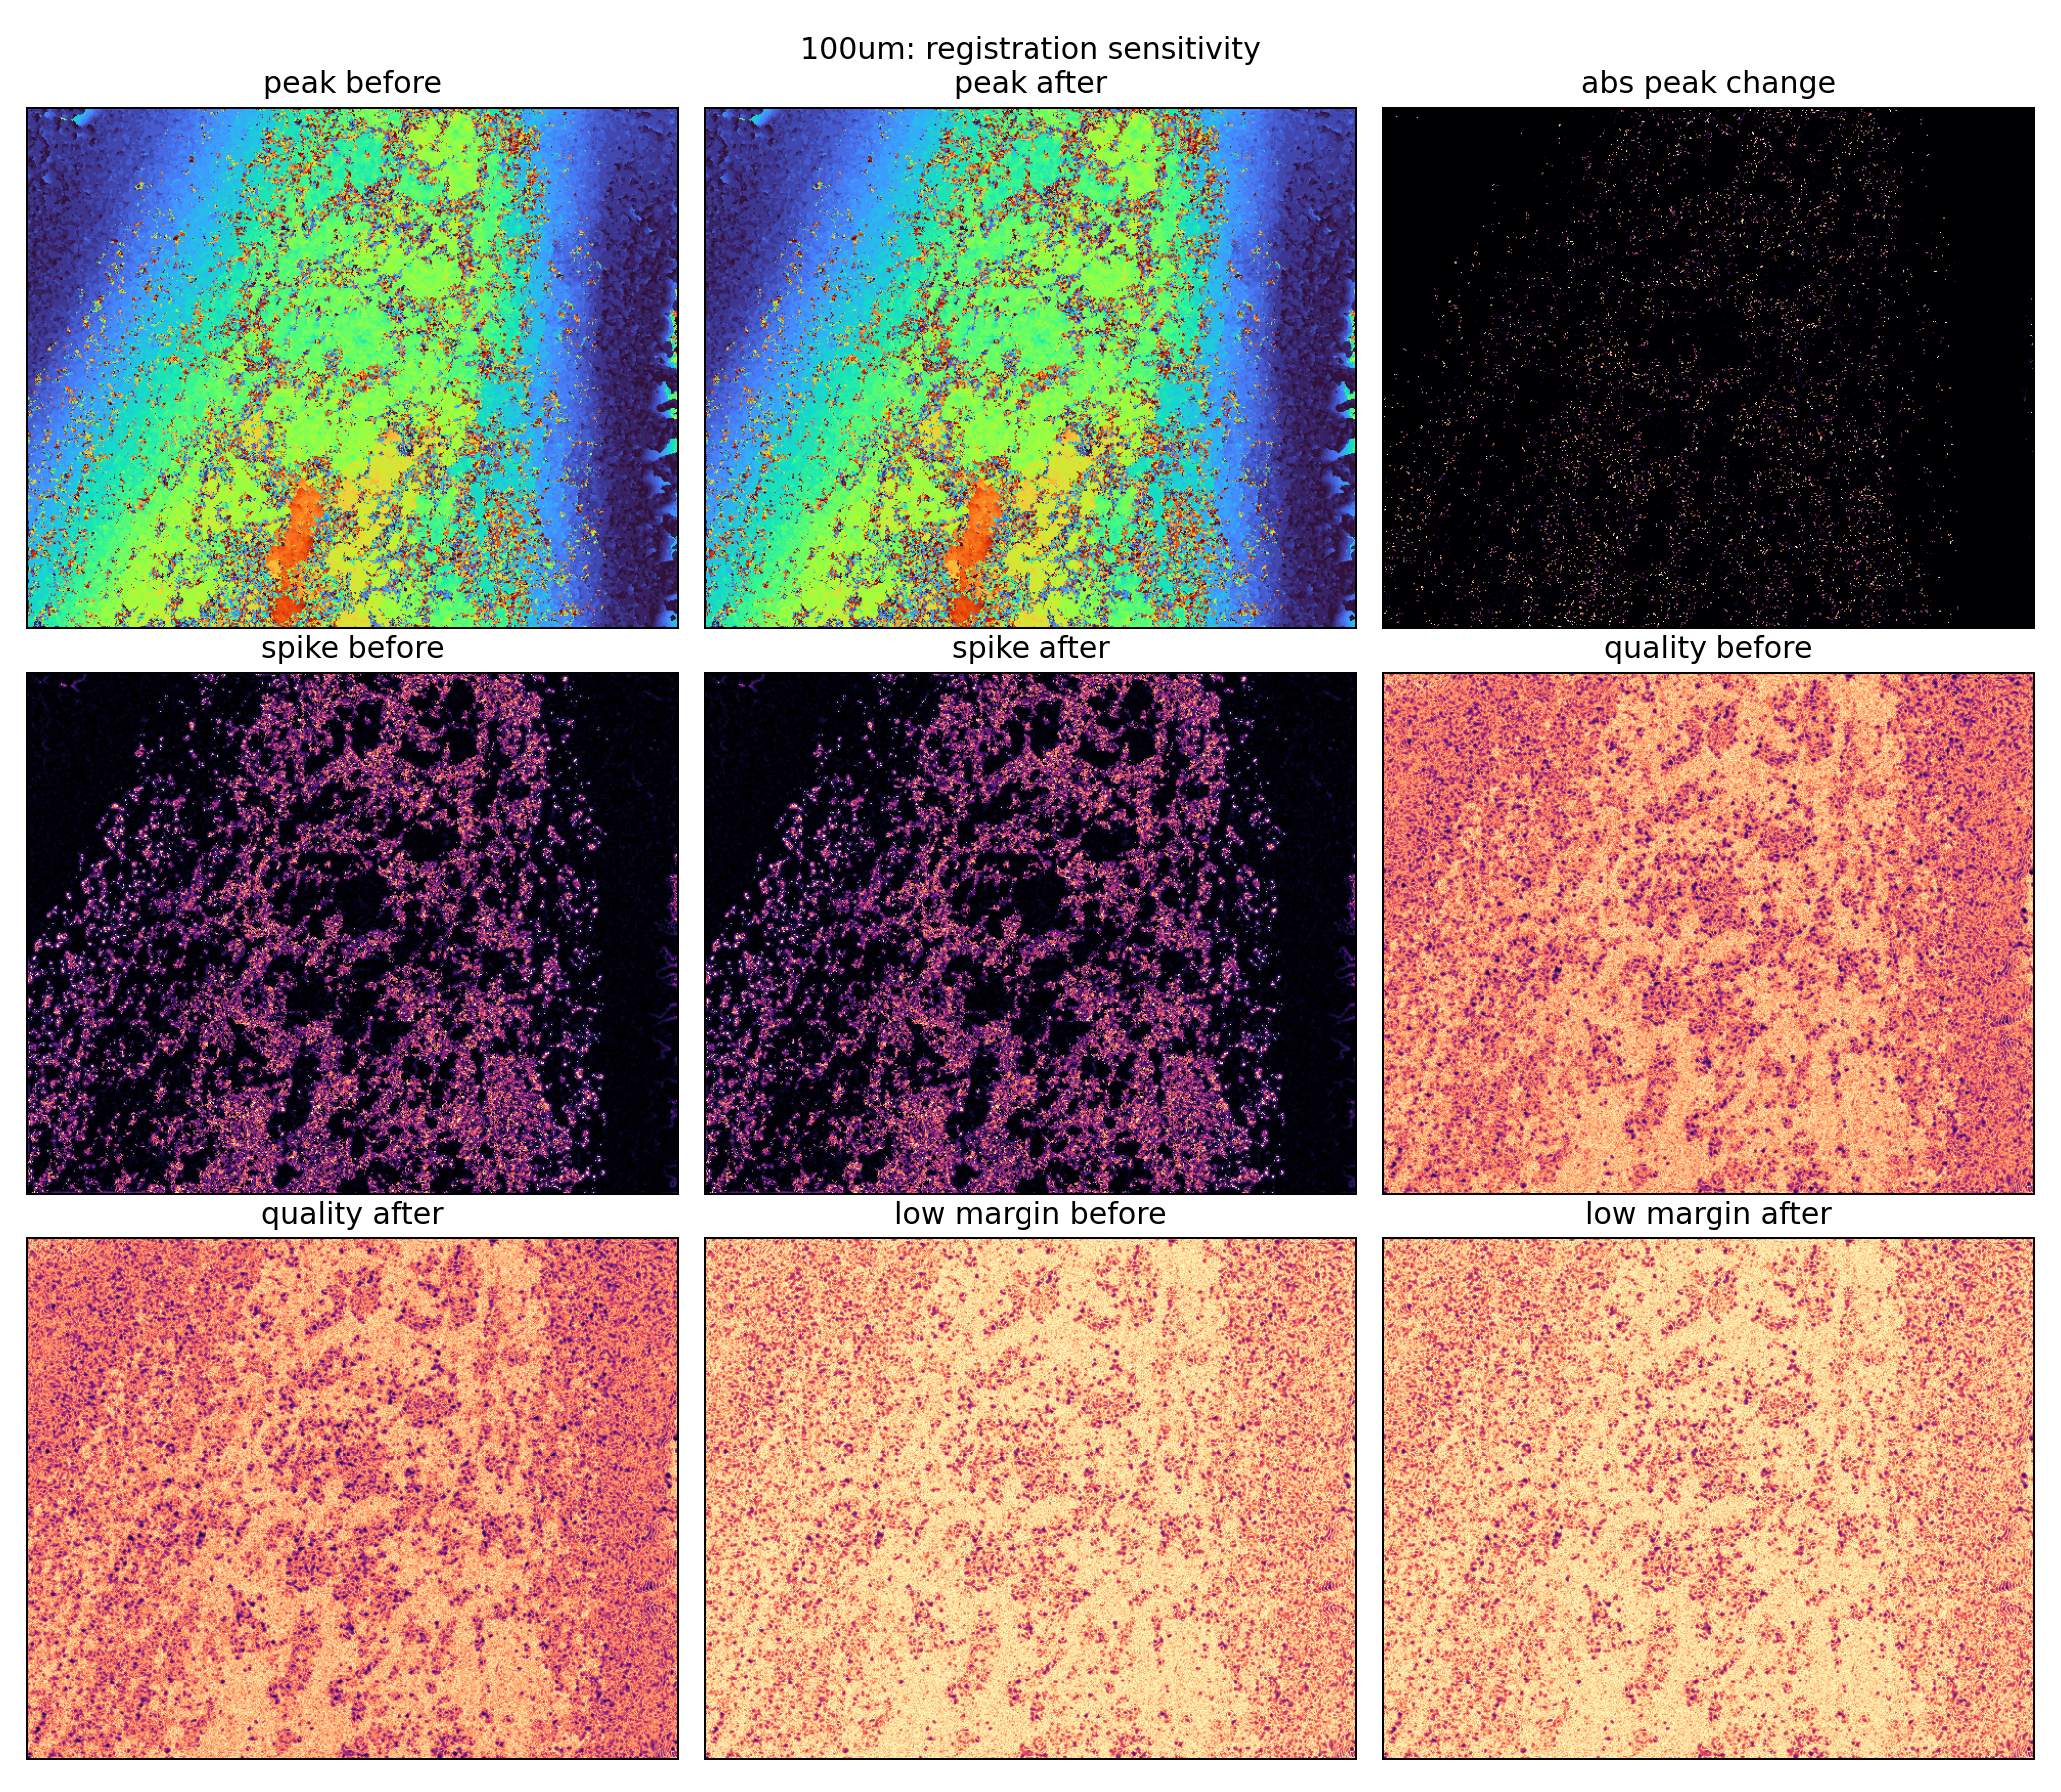
\includegraphics[width=\linewidth]{real_registration_probe/钥匙纹路100um_registration_sensitivity_maps.png}
\caption{Peak-layer, spike-proxy, quality-proxy, and low-margin maps before and after translation compensation.}
\end{figure}

\section{Interpretation}

配准估计的最大位移只有 0.1118 px，且大部分层位移为 0。配准后，只有 4.68\% 像素的 DFF peak layer 发生变化，90\% 像素的 peak layer 变化为 0。说明当前真实焦栈中的大面积 peak-layer 结构和主要散点分布在全局平移校正后仍然保留。

配准前后 spike proxy 的 Pearson 相关为 0.9478，quality proxy 的 Pearson 相关为 0.9825。更关键的是，\texttt{low\_margin} 对 spike top10 的 AUC 从 0.7293 变为 0.7287，几乎不变；组合 \texttt{quality\_proxy} 对 spike top10 的 AUC 从 0.9289 变为 0.9299。这说明上一轮“focus confidence 能定位真实焦栈中 DFF 层选择局部不稳定区域”的结论，对小幅全局平移配准不敏感。

\section{Paper-Ready Statement}

To evaluate whether the real-stack diagnostics are dominated by inter-layer translation, we estimate global shifts using phase cross-correlation with layer 20 as the reference. The maximum estimated shift magnitude is only 0.1118 pixels, with a median of 0 pixels. After translation compensation, only 4.68\% of pixels change their selected DFF peak layer. The spike-proxy map remains highly correlated with the original map (Pearson = 0.9478), and the quality-proxy map is even more stable (Pearson = 0.9825). The AUC of the low-margin score for identifying top 10\% spike-proxy pixels changes from 0.7293 to 0.7287. These results indicate that the observed focus-response instability and local DFF layer-selection jumps cannot be explained by small global frame shifts alone.

\section{Limitations}

本轮只估计二维全局平移，且使用中心区域做相位相关。它不能排除层间放大率变化、非刚性局部形变、主光线方向变化、入瞳或照明锥角变化，以及由于离焦导致的结构外观变化。因此，本结果应作为“全局平移不足以解释现象”的证据，而不应写成“已完全排除所有采集几何误差”。

\end{document}
